\documentclass[11pt]{article}
\usepackage[utf8]{inputenc}
\usepackage[T1]{fontenc}
\usepackage{lmodern}
\usepackage[a4paper,margin=2.5cm]{geometry}
\usepackage{setspace}
\usepackage{graphicx}
\usepackage{array}
\usepackage{tabularx}
\usepackage{booktabs}
\usepackage{xcolor}
\usepackage{lineno}
\usepackage[hidelinks]{hyperref}
\usepackage{xurl}
\DeclareUnicodeCharacter{2212}{\ensuremath{-}}
\newcommand{\todo}[1]{\textcolor{red}{#1}}
\newcolumntype{L}[1]{>{\raggedright\arraybackslash}p{#1}}
\renewcommand{\tabularxcolumn}[1]{>{\raggedright\arraybackslash}p{#1}}
\setlength{\tabcolsep}{4pt}
\onehalfspacing
\linenumbers

\title{Reproducibility practice in medical and life-science papers at top machine-learning venues and their agentic reproduction: a systematic meta-research study}
\author{Ekaterina Kondrateva\textsuperscript{1,2}, Florian Kofler\textsuperscript{1,3,4,5}, Attila Simkó\textsuperscript{6}}
\date{}
\begin{document}
\maketitle
\begin{flushleft}\small
\textsuperscript{1} Hertie AI Institute for Brain Health, University of Tübingen, Tübingen, Germany \\ \textsuperscript{2} Maastricht University, Maastricht, the Netherlands \\ \textsuperscript{3} University of Zurich, Zurich, Switzerland \\ \textsuperscript{4} Technical University of Munich, Munich, Germany \\ \textsuperscript{5} Helmholtz Munich, Munich, Germany \\ \textsuperscript{6} Umeå University, Umeå, Sweden \\ Corresponding author: Ekaterina Kondrateva, ekaterina.kondrateva@maastrichtuniversity.nl. ORCID 0000-0003-3623-6106.
\end{flushleft}
\section*{Abstract}
\textbf{Background.} Medical machine-learning (ML) papers are often assumed to be hard to reproduce because their data are restricted and their code is not shared. Agentic reproduction, in which AI agents attempt to rerun published work, now makes it possible to test this at conference scale.

\textbf{Methods.} We drew all 2,170 papers labelled clinical or life science (together, medical papers) by blind language-model coders (Cohen's kappa 0.96) from nine venue-years of CVPR, ICCV, ECCV, ICLR, ICML and NeurIPS (2025 to 2026), and an equal random sample of other papers. One language-model coder read all 3,278 full texts we could retrieve and a second, blind coder a random 25\%, under a protocol frozen before data collection; twelve reproducibility practices were coded. Differences were pooled across venue-years with Mantel-Haenszel risk differences and paper bootstrap intervals. Reproduction outcomes came from the public verdicts of the ICML 2026 agent reproduction challenge.

\textbf{Results.} Among papers that stated each practice, medical papers released code in 59\% versus 46\% (pooled difference +13 points, 95\% CI +10 to +17), reported variance in 66\% versus 42\% (+24, +21 to +28) and reported openly available main data more often (+15, +11 to +19). Restricted to empirical papers the differences were smaller but held (code +11, +6 to +15; open data +7, +2 to +12). Releases of weights, outputs and sample data were rarely stated by either group, and few papers listed their main claims with each tied to a specific table, figure or theorem (2.7\% of medical versus 6.1\% of other papers). In the challenge, attempted medical papers received a verified or falsified verdict 19 points less often than 1,821 other attempted papers (CI −28 to −10; permutation p < 0.001), mainly clinical papers, and their undecided claims were mostly rated inconclusive (49\% versus 25\% of claims). Within the same team, claims were decided about equally often (−3.6, −7.8 to +0.8). Medical papers were first taken up by teams that settled fewer of their other papers (40\% versus 60\%). Adjusting for this first-team strength removed the gap in being decided (−3.6, −12 to +5) but not in full verification (−12, −15 to −8). In a subsample of 220 papers whose claims were coded, medical claims more often needed retraining or large-scale runs (57\% versus 39\%), and adjusting for both factors reduced the full-verification gap to −6 (−12 to +1). Stated practices predicted poorly what reproducers obtained (code: kappa 0.22).

\textbf{Conclusions.} Medical papers at top ML venues are not less documented than other papers. In crowd reproduction they are settled less often, and the gap follows the teams that take them up and, in part, the cost of checking their claims. Authors should state their main claims explicitly and tie each one to the specific result that supports it, and reproduction efforts should report who attempted each paper and what its claims cost to check.

\section*{Introduction}
Concerns about the reproducibility of medical artificial intelligence are long-standing. When a high-profile study of AI for breast cancer screening was published without its code and with few methodological details, critics argued that this undermined its scientific value~\cite{r1}. A survey of 511 papers found that ML for health compared poorly with other areas of ML on dataset and code accessibility~\cite{r2}. In the radiology journals of the RSNA, 34\% of 218 AI articles shared code and 11\% shared code that reproduced~\cite{r3}, and at the Medical Imaging with Deep Learning conference only 22\% of accepted full papers from 2018 to 2022 had a repository judged repeatable~\cite{r4}. An audit of 400 AI conference papers found that none documented all the variables a reproduction needs~\cite{r5}. NeurIPS responded with a code submission policy, a reproducibility checklist and a community-wide reproducibility challenge~\cite{r6}, and failures such as data leakage have been traced across 17 fields that apply ML~\cite{r7}.

These studies measure what authors state. Whether stated materials let a third party settle a paper's claims is a different question, and until recently it could not be asked at scale, because each reproduction took weeks of expert work. AI agents now attempt reproductions of whole papers~\cite{r8}. In 2026 the International Conference on Machine Learning (ICML) ran an open agent reproduction challenge in which more than 1,200 participants published 6,816 reproduction logbooks on 2,226 conference papers, and an automated judge rated 35,908 claims as verified, falsified, toy (evidence at reduced scale) or inconclusive~\cite{r9}. This gives, for one venue, an outcome for reproduction that does not depend on what authors say about their own work.

We asked two questions. First, do medical papers at top ML venues state reproducibility practices less often than other papers, as is commonly assumed? Second, in the ICML 2026 challenge, are medical papers settled (verified or falsified) as often as other papers, and if not, why? An earlier protocol of ours on the venue listings (Protocol 7, Supplementary File S1) had already found that medical papers declare a code link in the venue metadata more often than other papers (24.5\% versus 16.9\% across twelve venue-years, +7.4 points, 95\% CI +5.8 to +9.0). For the practices that the metadata does not show (open data, weights and variance), we nonetheless prespecified the common assumption, that medical papers report them less often, as directional hypotheses. The full texts showed the opposite, and the outcomes showed a gap in the other direction, which we then examined with post hoc analyses whose reading rules were fixed before computing.

\section*{Methods}
The study followed a protocol frozen in a public repository before any data were collected, and is reported following the PRISMA 2020 statement~\cite{r10} where its items apply to a meta-research study of published papers. The protocol, its amendments and the reporting checklist are described in Appendix A.

\subsection*{Information sources and eligibility}
The sources were the public virtual-site listings of nine venue-years: CVPR 2025, ICCV 2025, ECCV 2026, ICLR 2025, ICLR 2026, ICML 2025, ICML 2026, NeurIPS 2025 and NeurIPS 2026 (40,290 papers after removing duplicates and papers without an abstract). Abstracts missing from the 2026 listings were taken from the challenge's paper metadata (ICML 2026) or from each paper's page on the venue site (ICLR 2026, NeurIPS 2026, ECCV 2026).

A paper was a candidate for the medical group if its venue topic was a health, biology, neuroscience or chemistry topic, or its title or abstract matched a prespecified regular expression of clinical and biological terms (Supplementary File S1, Protocol 7). This gave 5,530 candidates. Each candidate was labelled \texttt{clinical}, \texttt{life\_science} or \texttt{no} from title and abstract only by a blind language-model coder; a second blind coder labelled a random 25\% of candidates (1,633 papers over the whole listing; agreement 97.7\%, Cohen's kappa 0.96~\cite{r11}; gate 0.80) and disagreements were adjudicated with a written reason. Of the candidates, 1,013 were labelled clinical and 1,157 life science, together the 2,170 medical papers, and 3,360 were excluded. To estimate how many medical papers the prefilter missed, both coders labelled a random 200 non-candidates; none was medical (0 of 200, 95\% Wilson interval~\cite{r12} 0 to 1.9\%). The comparison group was a random sample of 2,170 non-candidates, allocated to venue-years in proportion to the medical counts (seed 20261019).

\subsection*{Full-text retrieval and excerpts}
Full texts were retrieved in a fixed order: arXiv HTML, then arXiv PDF (arXiv identifier from a title search, accepted at a normalised title similarity of at least 0.95 and an arXiv year no earlier than the venue year minus one; ambiguous matches excluded), then the open proceedings (CVF, PMLR). OpenReview was not scraped. Papers without a full text were counted and not imputed. From each full text an excerpt of at most 15,000 characters was built from the end of the introduction, sections whose heading concerned availability, reproducibility, ethics, data, setup, implementation, training, compute or limitations, the NeurIPS checklist items on reproducibility, and paragraphs on seeds and repeated runs, with a truncation flag per paper.

\subsection*{Data items and coding}
Each excerpt was coded on twelve fields (Table 1 lists the indicators): whether main claims were listed and linked to evidence; code (released, promised, no); main data access (open, credentialed or on request, private, synthetic only); an experiment on open data; release of synthetic or sample data, of weights and of outputs; variance (several seeds, error bars or intervals); environment (versions or container); compute (amount, hardware only, none); compute tier; and training-set scale. Every field allowed \texttt{unclear}. Coders used stated text only; a named dataset without stated access terms was \texttt{unclear}.

\begin{table}[htbp]
\centering\footnotesize
\renewcommand{\thetable}{1}
\caption{Medical papers state most reproducibility practices more often than other papers; only linking claims to results is rarer. Practices stated in the full text, medical versus other papers, nine venue-years. Shares among papers with a known value; pooled difference is the Mantel-Haenszel risk difference over venue-years with a 95\% paper bootstrap interval.}\label{tab:table1}
\begin{tabularx}{\textwidth}{XL{1.75cm}L{1.75cm}L{3.55cm}L{1.75cm}}
\toprule
\textbf{Practice} & \textbf{Medical, \% (n known)} & \textbf{Other, \% (n known)} & \textbf{Pooled difference, points (95\% CI)} & \textbf{Unclear, medical / other} \\ \midrule
Main claims listed and linked to evidence & 2.7 (1542) & 6.1 (1690) & −3.3 (−4.7 to −1.9) & 26 / 20 \\
Code released & 59.4 (1471) & 46.2 (1618) & +13.1 (+9.6 to +16.6) & 97 / 92 \\
Main data openly available & 83.7 (866) & 67.3 (627) & +15.0 (+10.7 to +19.3) & 702 / 1083 \\
Experiment on open data & 91.2 (1009) & 76.6 (901) & +13.3 (+10.2 to +16.4) & 559 / 809 \\
Synthetic or sample data released & 20.8 (173) & 11.1 (450) & +9.7 (+2.9 to +16.3) & 1395 / 1260 \\
Weights released & 48.6 (280) & 19.4 (495) & +28.6 (+21.6 to +35.0) & 1288 / 1215 \\
Outputs released & 19.7 (157) & 9.0 (422) & +12.5 (+6.2 to +19.5) & 1411 / 1288 \\
Variance reported & 66.4 (1269) & 42.1 (1372) & +24.4 (+20.7 to +27.9) & 299 / 338 \\
Environment stated & 16.9 (670) & 8.8 (880) & +8.5 (+5.1 to +11.8) & 898 / 830 \\
Compute amount stated & 21.7 (1113) & 17.1 (1332) & +5.2 (+2.0 to +8.2) & 455 / 378 \\
\bottomrule
\end{tabularx}
\end{table}

Coding was done by language-model subagents (claude-sonnet-5-5), 20 papers per batch, with venue, year and group hidden. Coder 1 coded all papers and coder 2 a random 25\% (813 papers). The protocol set a gate of kappa 0.80 on each primary field (code, main data access, weights, variance, compute). Code (0.85), main data access (0.83) and weights (0.96) met the gate and use coder 1's codes. Variance (0.71) and compute (0.70) did not; as the protocol required, coder 2 then coded these two fields for all papers and every disagreement (1,404 items) was adjudicated by a blind adjudicator (claude-opus-5-5) who saw the two labels in random order and gave a reason.

\subsection*{Reproduction outcomes}
Outcomes came from the public verdict snapshot of the ICML 2026 agent reproduction challenge retrieved on 17 October 2026~\cite{r9}. In the challenge, participants chose papers from the conference list, for each of which the organisers had extracted core claims from the abstract as checkable targets, and reproduced them with AI agents, with or without human steering, on compute credits provided by the organisers~\cite{r9}. Each attempt was published as a logbook (a Trackio Space with the write-up, the code that ran, the artifacts it produced and, optionally, the agent's execution trace)~\cite{r9}. An automated judge (GLM-5.2) then read each logbook, treated the logbook's own self-assessment as untrusted, and gave each claim one of four verdicts: verified, falsified, toy (supported only by a reduced-scale or synthetic-data run) or inconclusive; the organisers re-checked every claimed falsification themselves~\cite{r9}. On fixed input this judge agreed with itself well (Krippendorff's alpha 0.874), whereas verdicts on the same claim from different logbooks agreed poorly (alpha 0.229), a difference its author attributes mainly to the evidence that different attempts produce rather than to the judge~\cite{r13}.

A paper was attempted if it had at least one logbook, decided if at least one of its claims was rated verified or falsified, and fully verified if some logbook verified every claim it rated. Logbooks were deduplicated, and the first author's own logbooks were excluded because the first author took part in the challenge. Of the 6,341 ICML 2026 papers, 622 candidates labelled \texttt{no} were excluded, leaving 328 medical and 5,391 other papers.

To test whether stated practices agree with what reproducers obtained (reference standard), two blind coders read the logbooks of the 222 attempted ICML 2026 papers in the frame and coded whether the authors' code was obtained and run, the main data obtained, and weights used; disagreements were adjudicated as above. A further random 300 attempted ICML 2026 papers outside the frame were added later under a prespecified extension (Note 9-17).

\subsection*{Quantitative synthesis}
For each indicator we computed the share of papers with the practice among papers with a known value (\texttt{unclear} excluded and counted), by group and venue-year, with Wilson intervals~\cite{r12}. The difference between groups was pooled over the nine venue-years as a Mantel-Haenszel risk difference~\cite{r14}, with a 95\% interval from 2,000 paper bootstrap resamples within strata (seed 20261017; results identical under two hash seeds). Three directional hypotheses were prespecified: medical papers report open main data, release weights and report variance less often; each was to be accepted only if the pooled interval excluded zero in that direction.

For reproduction outcomes the primary analysis compared the decided share of attempted papers by group, unadjusted and adjusted for compute tier and data scale. Post hoc analyses (Notes 9-9 to 9-15), each with its reading rule frozen before computing, examined how many teams attempted each paper, the strength of the first team (the share of its other attempted papers on which its own latest logbook was decided, the paper itself left out), within-team claim-level differences, and the cost of checking each claim. For the last, two blind coders labelled every distinct claim text of the 110 attempted medical papers and of 110 randomly drawn attempted other papers as needing inference only, retraining, large-scale runs, or analysis only; the claim texts reveal the subject, so these coders were blind to the group label but not to the domain. An adjustment was read as accounting for a gap if the adjusted estimate was less than half the unadjusted one and its interval included zero. Adversarial checks (Notes 9-12 and 9-14) stated in advance what would refute each main claim. After an internal review of this manuscript, three further post hoc analyses were frozen before their intervals were computed (Note 9-22): documentation differences among empirical papers only (papers that stated a training-set size), release fields with \texttt{unclear} counted as not released, and the mix of verdicts by group. We did not correct for multiple comparisons; the post hoc analyses are exploratory.

\subsection*{Ethics}
The study used published papers and public challenge records, and involved no human participants and no patient data. The challenge records include the public account names under which participants published their logbooks. We used them only to group logbooks by team; no account name is reported in this paper or in the paper-level table. No ethics review was sought for this secondary analysis of public records.

\section*{Results}
Figure 1 summarises the main results.

\begin{figure}[htbp]
\centering
\setcounter{figure}{0}
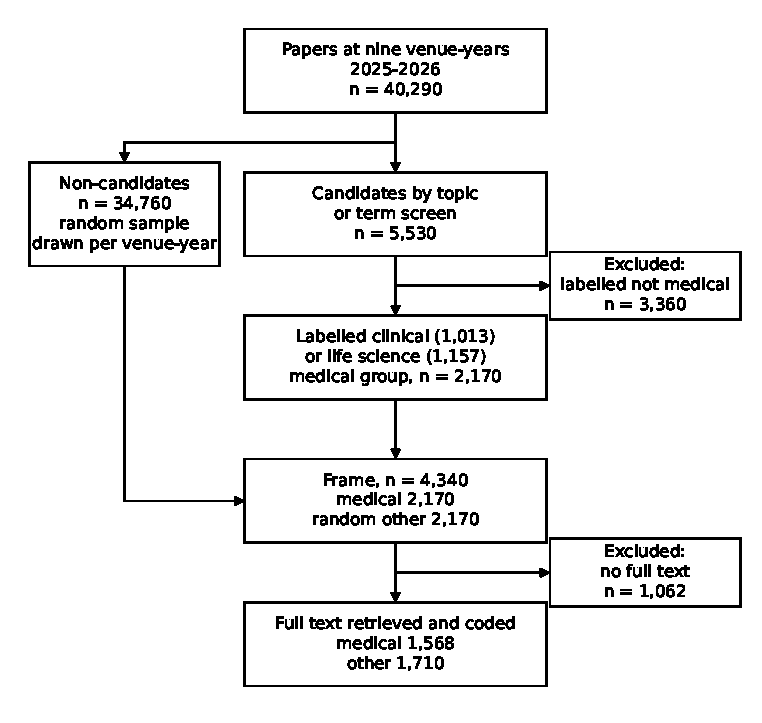
\includegraphics[width=\textwidth]{figures/fig1.pdf}
\caption{Medical papers state more but are settled less often, and the gap follows who takes them up. (a) Among papers that stated each practice, medical papers (orange) released code, reported open main data and reported variance more often than other papers (blue); both groups rarely tied their claims to a specific result. (b) In the ICML 2026 challenge, attempted medical papers were decided less often, with fewer claims verified and more rated inconclusive. (c) The decided gap disappears within the same team and after adjusting for the strength of the first team to take a paper up; the full-verification gap needs claim cost as well. Filled circles: interval excludes zero; open circles: interval includes zero. (d) What a paper states agrees poorly with what reproducers obtained; the dashed line marks kappa 0.40.}\label{fig:1}
\end{figure}

\subsection*{Study selection}
Figure 2 shows the flow of papers. Of the 4,340 papers in the frame, full texts were retrieved for 3,278 (1,568 medical and 1,710 other papers); 1,057 could not be matched to a full text, 4 failed to download and 1 had no usable text. Retrieval was complete or nearly complete for ICML, CVPR and ICCV, which have open proceedings, and lowest for NeurIPS 2026 (165 of 431 medical and 212 of 431 other papers) and the other venue-years that relied on arXiv alone (Table A1). It was lower for medical than for other papers (72.3\% against 78.8\%). Of the excerpts, 2,793 reached the 15,000-character cap.

\begin{figure}[htbp]
\centering
\setcounter{figure}{1}
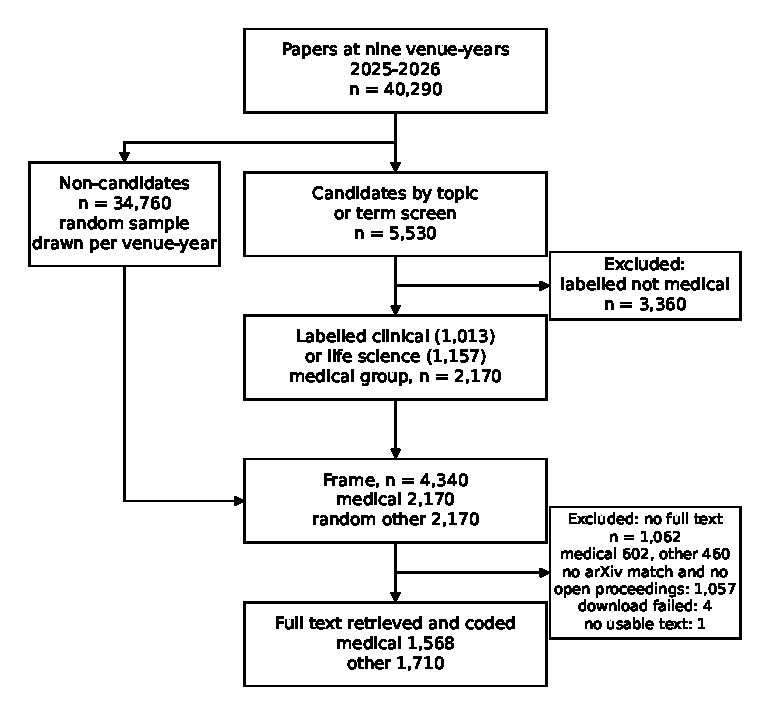
\includegraphics[width=\textwidth]{figures/fig2.pdf}
\caption{Most of the frame was coded, but a quarter had no retrievable full text, more often for medical papers. Flow of papers through the study; counts per venue-year are in Table A1.}\label{fig:2}
\end{figure}

\subsection*{Documentation practices}
Table 1 and Figure 3 give every indicator. Among papers with a known value, medical papers stated nine of the ten practices more often than other papers. They released code in 59.4\% of papers with a known value against 46.2\% (pooled difference +13.1 points, 95\% CI +9.6 to +16.6), reported open main data in 83.7\% against 67.3\% (+15.0, +10.7 to +19.3), released weights in 48.6\% against 19.4\% (+28.6, +21.6 to +35.0) and reported variance in 66.4\% against 42.1\% (+24.4, +20.7 to +27.9). None of the three prespecified hypotheses was accepted: all three differences ran in the opposite direction. The exception was claims listed and each tied to a table, figure or theorem, which was rare in both groups (2.7\% against 6.1\%, −3.3 points, −4.7 to −1.9). Compute was rarely stated by either group (21.7\% and 17.1\% gave an amount), and most papers did not state their compute tier (1,349 of 1,568 medical papers).

\begin{figure}[htbp]
\centering
\setcounter{figure}{2}
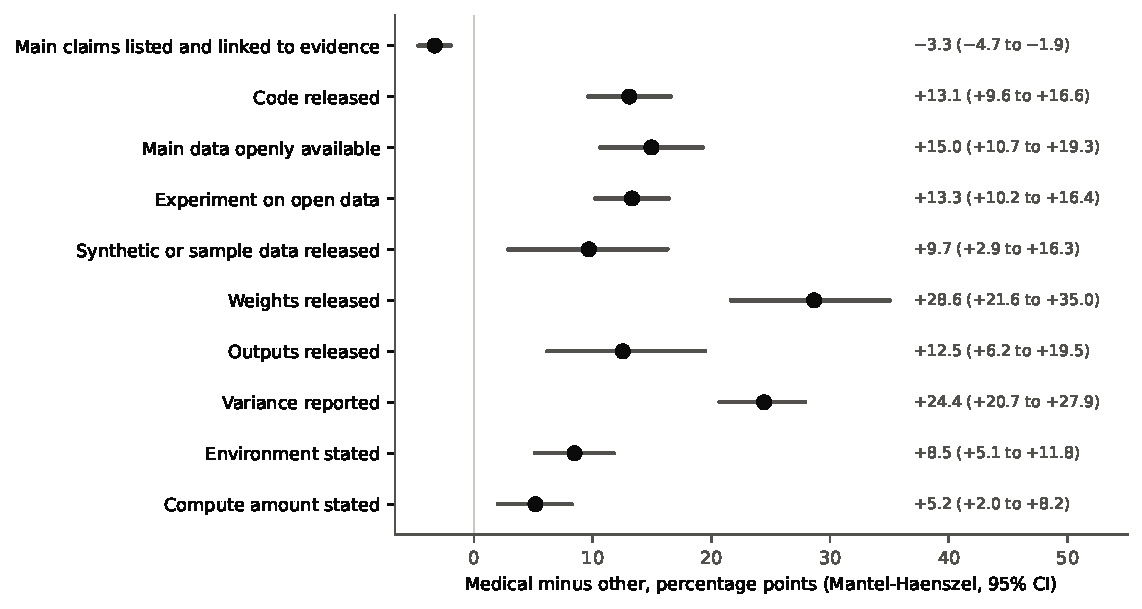
\includegraphics[width=\textwidth]{figures/fig3.pdf}
\caption{Medical papers state nine of ten practices more often than other papers; only linking claims to results is rarer. Mantel-Haenszel risk difference, medical minus other, over nine venue-years with 95\% bootstrap intervals, among papers with a known value. Filled circles: interval excludes zero.}\label{fig:3}
\end{figure}

The four main differences survived every prespecified check (Note 9-12, F1): leaving out each venue-year in turn, using coder 1's or coder 2's codes alone, restricting to papers whose excerpt was not truncated, and stratifying by venue-year and excerpt length. They held for clinical and life-science papers separately and for vision venues (CVPR, ICCV, ECCV) and learning venues (ICLR, ICML, NeurIPS) separately, except open main data at vision venues (+7.5, −1.9 to +16.9).

The comparison group contained more papers without an experiment on data: 43.7\% of other papers stated no training-set size, against 28.0\% of medical papers. Among the 1,129 medical and 962 other papers that stated one, the differences were smaller but all four held (Table 4): code +10.6 (+6.0 to +15.0), open main data +7.1 (+2.1 to +12.2), weights +21.7 (+12.7 to +30.7) and variance +24.7 (+20.1 to +29.3). Release fields were often not stated at all: a statement on weights could be coded for 280 of 1,568 medical papers. With unstated releases counted as none, medical papers still reported open main data more often (46.2\% against 24.7\%, +21.7, +18.4 to +24.7), but the weights difference fell to +3.1 points (+1.3 to +4.8), and the differences in synthetic or sample data (−0.6, −1.7 to +0.5) and outputs (−0.2, −1.2 to +0.8) disappeared.

\begin{table}[htbp]
\centering\footnotesize
\renewcommand{\thetable}{4}
\caption{The documentation differences hold among empirical papers; with unstated releases counted as none, only the open-data difference stays large. Medical minus other, Mantel-Haenszel over venue-years, points with 95\% CI (post hoc, Note 9-22).}\label{tab:table4}
\begin{tabularx}{\textwidth}{XL{3.55cm}L{3.55cm}L{3.9cm}}
\toprule
\textbf{Practice} & \textbf{Main analysis: known value} & \textbf{Empirical papers only: known value} & \textbf{All coded papers, unclear counted as none} \\ \midrule
Code released & +13.1 (+9.6 to +16.6) & +10.6 (+6.0 to +15.0) &  \\
Main data openly available & +15.0 (+10.7 to +19.3) & +7.1 (+2.1 to +12.2) & 46.2 vs 24.7\%; +21.7 (+18.4 to +24.7) \\
Weights released & +28.6 (+21.6 to +35.0) & +21.7 (+12.7 to +30.7) & 8.7 vs 5.6\%; +3.1 (+1.3 to +4.8) \\
Variance reported & +24.4 (+20.7 to +27.9) & +24.7 (+20.1 to +29.3) &  \\
Synthetic or sample data released & +9.7 (+2.9 to +16.3) &  & 2.3 vs 2.9\%; −0.6 (−1.7 to +0.5) \\
Outputs released & +12.5 (+6.2 to +19.5) &  & 2.0 vs 2.2\%; −0.2 (−1.2 to +0.8) \\
\bottomrule
\end{tabularx}
\end{table}

\subsection*{Reproduction outcomes in the ICML 2026 challenge}
Medical papers were attempted about as often as other papers (110 of 328, 33.5\%, against 1,821 of 5,391, 33.8\%) but by fewer teams (mean 1.5 against 3.3 teams per attempted paper). Among attempted papers, 46.4\% of medical papers were decided against 65.5\% of other papers, a difference of −19.1 points (95\% CI −28.4 to −9.6; permutation p < 0.001). The gap was larger for clinical papers (−23.6, −36.2 to −10.9) than for life-science papers (−13.4, −27.5 to +0.9), and it remained when every logbook of the team with the most medical attempts was dropped (−19.1, −29.7 to −8.7). The same direction held for full verification (−19.3, −22.1 to −15.7) and for any falsified claim (−10.8, −16.9 to −4.1). Claims of medical papers were rated verified in 21.7\% against 49.7\% and inconclusive in 49.2\% against 24.8\%; toy verdicts were about as common (25.5\% against 20.9\%, +4.7, −0.6 to +10.7). In the prespecified analysis on the 222 attempted frame papers, the gap was −17.0 points (−29.7 to −4.4); adjusting for stated compute tier and data scale left it at −14.7 (−28.8 to −0.5), so scale did not account for it.

Table 2 and Figure 4 show the post hoc decomposition. The judge did not treat medical claims differently: within the same team, claims of medical papers were decided 3.6 points less often than claims of other papers (−7.8 to +0.8), against 29.1 points less often without this adjustment. The first team to take up a medical paper had settled 40.0\% of its other attempted papers, against 60.3\% for teams first on other papers (−20.3, −26.0 to −14.3). Team strength behaved as a property of the team: on 903 papers attempted by at least two teams, the stronger team decided the same paper 32.3 points more often than the weaker one (+29.9 to +34.7). Adjusting for first-team strength reduced the decided gap from −19.1 to −3.6 points (−11.9 to +5.1), which meets the reading rule. It did not account for full verification: on all attempted papers that gap was −11.7 points (−14.7 to −8.0) after the adjustment. Whether a paper listed and linked its claims did not account for the decided gap either (adjusted −15.3 points, −28.5 to −2.2; 216 frame papers); few attempted papers in either group linked each claim to a result (3 medical and 9 other papers).

\begin{table}[htbp]
\centering\footnotesize
\renewcommand{\thetable}{2}
\caption{The gap in being decided disappears after adjusting for the strength of the first team; the gap in full verification needs claim cost as well. Reproduction outcomes of attempted ICML 2026 papers, medical minus other, unadjusted and adjusted (post hoc analyses, Notes 9-9 to 9-15).}\label{tab:table2}
\begin{tabularx}{\textwidth}{XL{3.6cm}}
\toprule
\textbf{Outcome and adjustment} & \textbf{Medical minus other, points (95\% CI)} \\ \midrule
Decided, all attempted papers (110 vs 1,821), unadjusted & −19.1 (−28.4 to −9.6) \\
Decided, clinical papers only & −23.6 (−36.2 to −10.9) \\
Decided, life-science papers only & −13.4 (−27.5 to +0.9) \\
Decided, adjusted for number of teams & −9.2 (−18.1 to +0.4) \\
Decided, adjusted for first-team strength & −3.6 (−11.9 to +5.1) \\
Fully verified, all attempted papers, unadjusted & −19.3 (−22.1 to −15.7) \\
Fully verified, all attempted papers, adjusted for first-team strength & −11.7 (−14.7 to −8.0) \\
Fully verified, claim-coded subsample (220 papers), unadjusted & −19.1 (−27.3 to −10.9) \\
Fully verified, subsample, adjusted for first-team strength & −13.0 (−20.7 to −5.1) \\
Fully verified, subsample, adjusted for strength and claim cost & −5.6 (−11.9 to +1.4) \\
Claim decided, unadjusted (claim level) & −29.1 (−37.9 to −20.2) \\
Claim decided, within team (claim level) & −3.6 (−7.8 to +0.8) \\
\bottomrule
\end{tabularx}
\end{table}

\begin{figure}[htbp]
\centering
\setcounter{figure}{3}
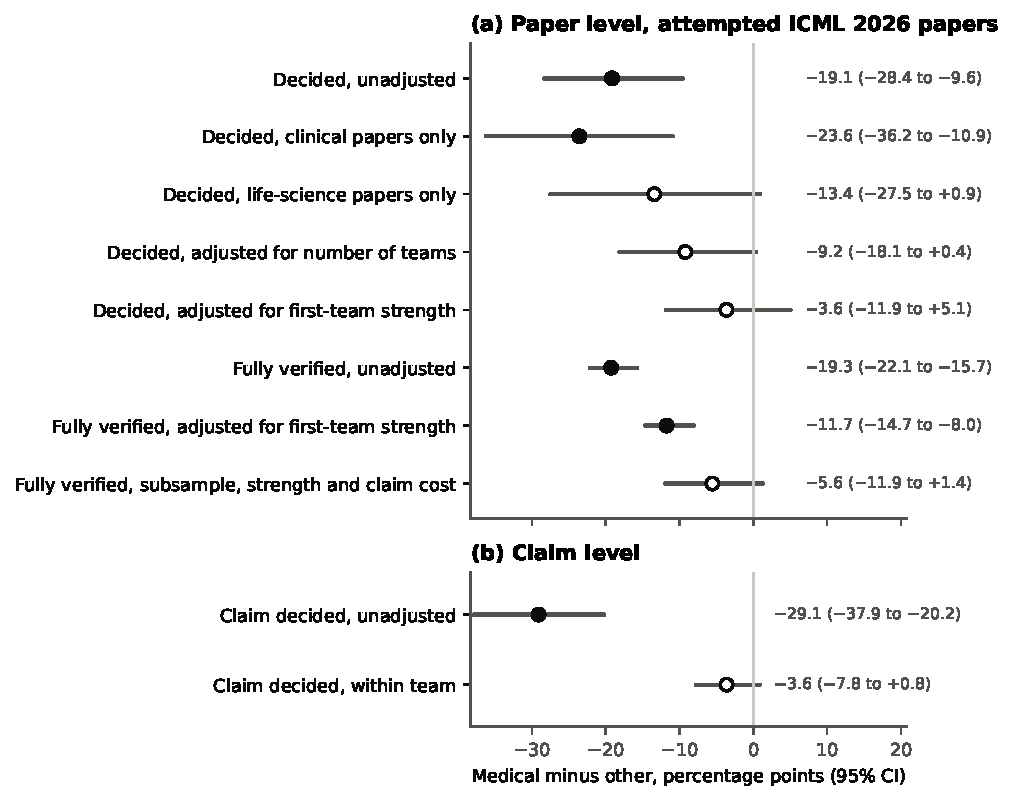
\includegraphics[width=\textwidth]{figures/fig4.pdf}
\caption{The gap in being decided disappears once team strength or team is accounted for; the gap in full verification also needs claim cost. Attempted ICML 2026 papers, medical minus other, with 95\% bootstrap intervals. (a) Paper level: decided and fully verified, unadjusted and adjusted. (b) Claim level: share of claims decided, unadjusted and within team. Filled circles: interval excludes zero.}\label{fig:4}
\end{figure}

Claims of medical papers were also costlier to check: of 1,083 claims coded in the subsample of 220 papers, 56.7\% of medical against 39.1\% of other claims needed retraining or large-scale runs (+17.6, +9.7 to +25.8), and fewer could be settled by analysis alone (19.3\% against 45.3\%). In this subsample, the full-verification gap was −19.1 points, −13.0 (−20.7 to −5.1) after adjusting for first-team strength, and −5.6 (−11.9 to +1.4) after adjusting for both strength and claim cost.

\subsection*{Stated practices against what reproducers obtained}
On the 222 attempted frame papers, a stated code release agreed poorly with reproducers having run the authors' code (sensitivity 0.74, specificity 0.56, kappa 0.22; n = 162 with a known value on both sides), and stated open data agreed poorly with reproducers having obtained the data (kappa 0.13, n = 89). Weights agreed better (kappa 0.55, n = 43). Pooled with the 300 extension papers, the kappas were 0.28 (n = 347), 0.16 (n = 163) and 0.60 (n = 118). In NeurIPS papers, the checklist answer on open code agreed with the coded code release at kappa 0.22 (n = 152) (Table 3).

\begin{table}[htbp]
\centering\footnotesize
\renewcommand{\thetable}{3}
\caption{What papers state agrees poorly with what reproducers obtained, except for weights. Agreement on the 222 attempted ICML 2026 frame papers; the last column pools them with the 300-paper extension sample.}\label{tab:table3}
\begin{tabularx}{\textwidth}{XL{0.7cm}L{1.6cm}L{1.6cm}L{1.0cm}L{2.4cm}}
\toprule
\textbf{Stated in full text vs obtained by reproducers} & \textbf{n} & \textbf{Sensitivity} & \textbf{Specificity} & \textbf{Kappa} & \textbf{Kappa pooled with extension (n)} \\ \midrule
Code released vs authors' code run & 162 & 0.74 & 0.56 & 0.22 & 0.28 (347) \\
Main data open vs data obtained & 89 & 0.87 & 0.27 & 0.13 & 0.16 (163) \\
Weights released vs weights used & 43 & 0.75 & 0.92 & 0.55 & 0.60 (118) \\
NeurIPS checklist item 5 vs code released & 152 & 0.80 & 0.53 & 0.22 &  \\
\bottomrule
\end{tabularx}
\end{table}

\section*{Discussion}
\subsection*{Principal findings}
Across nine venue-years of six top ML venues, medical papers stated code, open data and variance more often than other papers did, also among empirical papers only. This contradicts the assumption we set out to test. Weights and other releases were stated too rarely to compare. Yet in the one venue where outcomes could be observed, medical papers were settled less often by agentic reproducers, and their undecided claims were mostly inconclusive rather than checked at reduced scale. The gap was not in how the judge treated their claims. It went with which teams took the papers up: medical papers were taken up by fewer teams, first by teams that settled fewer papers of any kind, and this accounted for the gap in being decided at all. Team strength alone did not account for the gap in full verification. In a subsample of 220 papers, medical claims more often required retraining or large runs, and with both factors taken into account that gap fell from −19 to −6 points with an interval that included zero.

\subsection*{Comparison with earlier work}
An earlier survey found weaker sharing in ML for health than in other ML areas~\cite{r2}, and audits of medical imaging found low rates of shared and working code in radiology journals~\cite{r3} and at a medical imaging conference~\cite{r4}. Our frame differs: it covers only papers accepted at general ML venues, several of which have introduced code policies and checklists~\cite{r6}, and it compares medical papers with other papers at the same venues and in the same years. Within this setting the medical papers documented more. Earlier audits measured documentation alone~\cite{r5}, or tested whether shared code ran~\cite{r3,r4}; here documentation could be compared with what independent reproducers obtained, and a stated code link agreed with a reproducer actually running the authors' code at a kappa of only 0.22. PaperBench evaluated agents on a fixed set of 20 ICML 2024 Spotlight and Oral papers~\cite{r8}; in an open challenge, by contrast, participants choose what to attempt, and the challenge data show that the domain of a paper changes who attempts it and what is asked.

\subsection*{Implications}
The share of papers verified in a crowd reproduction depends on who attempts them and on what their claims cost to check, not only on what authors provide. A verified rate reported without these two factors would mislead readers about medical papers. Reporting guidelines for ML-based science~\cite{r15}, for clinical prediction models that use ML~\cite{r16} and for deep learning in medical imaging~\cite{r17} concern what authors state; at these venues medical papers already state more than others, and whether a crowd settles them depends on more than what is stated. The recommendations below follow from the measurements in this study; none of them was tested as an intervention.

\subsection*{Recommendations}
For authors of medical ML papers:

\begin{itemize}
\item State each main claim explicitly and tie it to the table, figure or theorem that supports it. Only 2.7\% of medical and 6.1\% of other papers did so, and the challenge organisers had to extract claims from abstracts instead~\cite{r9}.
\item State the access route of the main dataset in the paper (open, credentialed, on request or private), not only its name. Access could not be coded from the text for 702 of 1,568 medical papers.
\item State releases explicitly, including what is not released (weights, outputs, sample or synthetic data). Weights were unstated in 1,288 of 1,568 medical papers.
\item State the compute a claim needs (hardware and time). The compute tier was unstated in 1,349 of 1,568 medical papers, and medical claims more often needed retraining or large-scale runs.
\end{itemize}

For organisers of reproduction challenges and for logbook formats such as Trackio:

\begin{itemize}
\item Extract each claim together with the result it refers to (table, figure or theorem), so that a verdict is attached to a specific result rather than to a sentence of the abstract.
\item Record in each logbook, per claim, whether the authors' code was run, the main data obtained and the weights used. These facts had to be reconstructed from free text for the reference standard here, and they differed from what papers state.
\item Record what each check needed (inference only, retraining, large-scale runs) and the compute it used, and give a reason with every inconclusive verdict, since most undecided medical claims were inconclusive rather than toy.
\item Report per paper the number of teams that attempted it and their track record on other papers, and report domain comparisons adjusted for both, because the first team's strength alone accounted for the gap in being decided.
\end{itemize}

For venues:

\begin{itemize}
\item Ask authors to map each listed contribution to its supporting result in the reproducibility checklist, and to state data access and releases in fixed categories, because checklist answers agreed only moderately with the text (code: kappa 0.22).
\end{itemize}

\subsection*{Strengths and limitations}
The frame is a census of medical papers at nine venue-years with a matched comparison group, the protocol and coding rules were fixed before data collection, every coding decision is public, and the main documentation differences survived prespecified attempts to refute them. The study has several limitations. All coders, adjudicators and the challenge judge are language models; agreement between coders was high, but they may share systematic errors, and verdicts on the same claim from different logbooks agreed poorly in the challenge as a whole~\cite{r13}. The comparison group contains more papers without experiments, which explains part of the documentation differences, although all four main differences held among empirical papers. Full texts were missing for a quarter of the frame, mostly at NeurIPS 2026 and ICLR, where we relied on arXiv; retrieval was lower for medical papers, and papers posted on arXiv may document more than papers that are not. Many excerpts were truncated, so release fields are often \texttt{unclear}, and with \texttt{unclear} counted as none most release differences shrink or disappear. Coded practices are what authors state, not working artifacts. We did not characterise how teams reproduced papers: the agents, the degree of human steering and the compute they used vary across logbooks~\cite{r9} and were not coded, so first-team strength may partly stand for the method a team used. The reproduction outcomes come from one venue, one challenge and one judge model, and the challenge's participants chose what to attempt. Protocol 9 was designed after the results of earlier protocols on the same challenge were known, including the higher rate of code links in medical papers. The explanations of the outcome gap are post hoc, rest on a chain of analyses without correction for multiple comparisons, and use different samples for team strength (all attempted papers) and claim cost (220 papers); they should be read as exploratory. The analyses are observational.

\subsection*{Conclusions}
Medical papers at top ML venues are not less documented than other papers at the same venues, yet in agentic crowd reproduction they are settled less often. The gap follows the teams that take them up and, in part, the cost of their claims, not a lack of stated materials. Authors should state their main claims explicitly and tie each one to the specific result that supports it, and reports of crowd reproduction should state who attempted each paper and what its claims cost to check.

\section*{Declarations}
\textbf{Data availability.} The paper-level table (4,340 papers with identifiers, titles, group, full-text status and all codes), the claim codes, the frozen protocol and all aggregate results are available at \url{https://github.com/kondratevakate/life-science-at-ml-venues} \todo{[DOI to be added on release]} (code MIT licence; data and text CC BY 4.0). Abstracts and full texts were retrieved from public conference websites, arXiv and open proceedings and are not redistributed for copyright reasons; the repository contains the retrieval scripts and SHA-256 manifests of the retrieved files. Challenge verdicts come from the public snapshot of the ICML 2026 agent reproduction challenge retrieved on 17 October 2026. No patient data were used.

\textbf{Code availability.} All analysis code is in the repository above; \texttt{python setup\_data.py} links the retrieved inputs and each analysis script reproduces its result file. Rerunning all Protocol 9 analyses from the committed codes gave byte-identical results.

\textbf{Ethics approval and consent.} Not applicable: secondary analysis of published papers and public challenge records, with no human participants and no patient data. Public account names of challenge participants were used only to group logbooks by team and are not reported.

\textbf{Competing interests.} EK took part in the ICML 2026 agent reproduction challenge as a reproducer; her own logbooks were excluded from all analyses. \todo{[Other competing interests of all authors to be added.]}

\textbf{Funding.} \todo{[To be added.]}

\textbf{Author contributions.} \todo{[To be added in CRediT terms.]}

\textbf{Use of AI tools.} Paper labels, full-text codes, reference-standard codes, claim codes and adjudications were produced by language-model subagents (claude-sonnet-5-5 and claude-opus-5-5) under the frozen protocol and prompts, which are public in the repository. Analysis code and drafts of this manuscript were written with the assistance of Claude (Anthropic). The authors checked every number against the result files and take responsibility for the content.

\clearpage
\begin{thebibliography}{99}
\bibitem{r1} Haibe-Kains B, Adam GA, Hosny A, Khodakarami F, Massive Analysis Quality Control (MAQC) Society Board of Directors, Waldron L, et al. Transparency and reproducibility in artificial intelligence. Nature. 2020;586(7829):E14–6. doi:10.1038/s41586-020-2766-y
\bibitem{r2} McDermott MBA, Wang S, Marinsek N, Ranganath R, Foschini L, Ghassemi M. Reproducibility in machine learning for health research: still a ways to go. Sci Transl Med. 2021;13(586):eabb1655. doi:10.1126/scitranslmed.abb1655
\bibitem{r3} Venkatesh K, Santomartino SM, Sulam J, Yi PH. Code and data sharing practices in the radiology artificial intelligence literature: a meta-research study. Radiol Artif Intell. 2022;4(5):e220081. doi:10.1148/ryai.220081
\bibitem{r4} Simkó A, Garpebring A, Jonsson J, Nyholm T, Löfstedt T. Reproducibility of the methods in medical imaging with deep learning. In: Medical Imaging with Deep Learning. Proceedings of Machine Learning Research. 2024;227:95–106.
\bibitem{r5} Gundersen OE, Kjensmo S. State of the art: reproducibility in artificial intelligence. Proc AAAI Conf Artif Intell. 2018;32(1). doi:10.1609/aaai.v32i1.11503
\bibitem{r6} Pineau J, Vincent-Lamarre P, Sinha K, Larivière V, Beygelzimer A, d'Alché-Buc F, et al. Improving reproducibility in machine learning research (a report from the NeurIPS 2019 reproducibility program). J Mach Learn Res. 2021;22(164):1–20.
\bibitem{r7} Kapoor S, Narayanan A. Leakage and the reproducibility crisis in machine-learning-based science. Patterns. 2023;4(9):100804. doi:10.1016/j.patter.2023.100804
\bibitem{r8} Starace G, Jaffe O, Sherburn D, Aung J, Chan JS, Maksin L, et al. PaperBench: evaluating AI's ability to replicate AI research. In: Proceedings of the 42nd International Conference on Machine Learning. PMLR; 2025. p. 56843–73.
\bibitem{r9} Abid A. What we learned by reproducing 2,200 papers from ICML [Internet]. Hugging Face; 2026 Aug 13. Available from: \url{https://huggingface.co/blog/icml-2026-open-reproductions}
\bibitem{r10} Page MJ, McKenzie JE, Bossuyt PM, Boutron I, Hoffmann TC, Mulrow CD, et al. The PRISMA 2020 statement: an updated guideline for reporting systematic reviews. BMJ. 2021;372:n71. doi:10.1136/bmj.n71
\bibitem{r11} Cohen J. A coefficient of agreement for nominal scales. Educ Psychol Meas. 1960;20(1):37–46. doi:10.1177/001316446002000104
\bibitem{r12} Wilson EB. Probable inference, the law of succession, and statistical inference. J Am Stat Assoc. 1927;22(158):209–12. doi:10.1080/01621459.1927.10502953
\bibitem{r13} Umoh EH. Who verifies the verifier? Measuring LLM-as-judge reliability across 32,688 automated research verdicts \todo{[poster]}. AWS-MLU Fall AI Teaching and Research Symposium; 2026 Sep 22; Arlington, VA. Available from: \url{https://github.com/SturdivantAI/who-verifies-the-verifier}
\bibitem{r14} Mantel N, Haenszel W. Statistical aspects of the analysis of data from retrospective studies of disease. J Natl Cancer Inst. 1959;22(4):719–48. doi:10.1093/jnci/22.4.719
\bibitem{r15} Kapoor S, Cantrell EM, Peng K, Pham TH, Bail CA, Gundersen OE, et al. REFORMS: consensus-based recommendations for machine-learning-based science. Sci Adv. 2024;10(18):eadk3452. doi:10.1126/sciadv.adk3452
\bibitem{r16} Collins GS, Moons KGM, Dhiman P, Riley RD, Beam AL, Van Calster B, et al. TRIPOD+AI statement: updated guidance for reporting clinical prediction models that use regression or machine learning methods. BMJ. 2024;385:e078378. doi:10.1136/bmj-2023-078378
\bibitem{r17} Moassefi M, Singh Y, Conte GM, Khosravi B, Rouzrokh P, Vahdati S, et al. Checklist for reproducibility of deep learning in medical imaging. J Imaging Inform Med. 2024;37(4):1664–73. doi:10.1007/s10278-024-01065-2
\end{thebibliography}
\section*{Appendix A. Protocol and reporting}
The study followed a written protocol (Protocol 9) frozen in a public git repository before the paper frame was drawn, before any full text was retrieved and before any coding (commit 839281e in kondratevakate/icml-2026-repro, 19 October 2026, five minutes before the first full text was retrieved). The protocol builds on three earlier protocols in the same repository (Protocols 6 to 8, on the same challenge) and was designed after their results were known. Every later decision is recorded as a dated note in the protocol (Notes 9-1 to 9-22), written before the analysis it governs was computed; analyses beyond those in the protocol are reported as post hoc and exploratory. The study was not registered in a review register. We report it following the PRISMA 2020 statement~\cite{r10} where its items apply to a meta-research study of published papers; the completed checklist is Supplementary File S2. The protocol, all notes and their commit history are in Supplementary File S1 and the repository. Table A1 gives the papers in the frame and with a coded full text per venue-year.

\begin{table}[htbp]
\centering\footnotesize
\renewcommand{\thetable}{A1}
\caption{Full texts were nearly complete where open proceedings exist and missing most often at NeurIPS 2026. Papers in the frame and with a coded full text, by group and venue-year.}\label{tab:tablea1}
\begin{tabularx}{\textwidth}{XL{4.2cm}L{4.2cm}}
\toprule
\textbf{Venue-year} & \textbf{Medical: frame / full text} & \textbf{Other: frame / full text} \\ \midrule
cvpr-2025 & 108 / 108 & 108 / 107 \\
iccv-2025 & 104 / 103 & 104 / 104 \\
eccv-2026 & 129 / 81 & 129 / 96 \\
iclr-2025 & 222 / 153 & 222 / 173 \\
iclr-2026 & 309 / 218 & 309 / 230 \\
icml-2025 & 166 / 166 & 166 / 165 \\
icml-2026 & 328 / 328 & 328 / 328 \\
neurips-2025 & 373 / 246 & 373 / 295 \\
neurips-2026 & 431 / 165 & 431 / 212 \\
Total & 2170 / 1568 & 2170 / 1710 \\
\bottomrule
\end{tabularx}
\end{table}

\end{document}